\section{Измерение продольной поляризации $\Lambda_c \to \Lambda \pi$}

С помощью формализма спиральных амплитуд \textbf{\cite{Richman}} можно описать процесс 
$\Lambda_c \to \Lambda \pi$ и получить его угловое распределение с 
учётом продольной поляризации. На рис. \ref{def:val} показаны определения 
наблюдаемых величин. 

\begin{figure}[H]
    \centering
    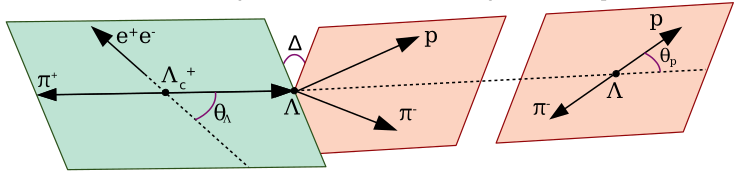
\includegraphics[width=0.7\linewidth]{img/lpi_def.png}
    \caption{Определение переменных.}
    \label{def:val}
\end{figure}

Амплитуда записывается следующим образом:

\begin{equation}
    A_{\llp{c} \llp{p}} = \sum_{\llp{c}} A_{\llp{c}} D^{1/2\dag}_{\llp{c} \llp{p}}\left(\phi_\lambda, \theta_\Lambda, -\phi_\Lambda \right) D^{1/2\dag}_{\llp{c} \llp{p}} B_{\llp{p}} D^{1/2}_{\llp{c} \llp{p}}\left(\phi_p, \theta_p, -\phi_p \right)
\end{equation}

Где $\llp{p}$ --- спиральность протона, 
$A_{\llp{c}}$ --- спиральная амплитуда $\Lambda_c \to \Lambda \pi^+$, 
$B_{\llp{c}}$ --- спиральная амплитуда $\Lambda_c \to \Lambda \pi^-$,
$\theta_\Lambda, \phi_\Lambda$ --- полярные углы импульса $\Lambda$ в системе $\Lambda_c$,
$\theta_p, \phi_\Lambda$ --- полярные углы импульса протона в системе $\Lambda$, 
$D^{j\dag}_{m' m}$ --- коэфиценты матрици Вигнера.

Угловое распределение, нормированное на единицу, в зависимости от
спиральности $\Lambda_c$-бариона:

\begin{equation}
    \cfrac{dW_{\llp{c}}}{d\cos{\theta_p}d\cos{\theta_p}d\phi_{\llp{c}}\phi_{\llp{p}}} = N \sum_{\llp{p}} \abs{A_{\llp{c} \llp{p}}}^2 
\end{equation}

Полное угловое распределение можно разложить по поляризациям

\begin{equation}
    dW = \cfrac{1+P_L}{2} dW_{+1/2} + \cfrac{1-P_L}{2} dW_{-1/2} 
\end{equation}

где $P_L$ — величина проекции вектора поляризации $\Lambda_c$-бариона 
на его импульс. После преобразований и сокращения общего множителя формула
углового распределения имеет вид:

\begin{equation}
    f_{sig}^{\Lambda\pi} \sim \cfrac{dW_{\llp{c}}}{d\cos{\theta_p}d\cos{\theta_p}d\phi_{\llp{c}}\phi_{\llp{p}}} 
    =
    1 + \alpha_{\Lambda}\alpha_{\Lambda_c} \cos \theta_p + 
    P\insqr{\cos\inner{\alpha_{\Lambda} + \alpha_{\Lambda_c} \cos{\theta_p}} - 
    \alpha_{\Lambda}\sqrt{1 - \alpha_{\Lambda_c}^2}\cos\inner{\delta + \Delta}\cos\theta_p \cos \theta_\Lambda}
\end{equation}

Где $\Delta = \phi_p - \phi_\Lambda$, 
$\arg\inner{A_{1/2}A_{-1/2}^\dag}$ --- фаза между спиральными амплитудами,
$\alpha_{\Lambda_c}$ и $\alpha_{\Lambda}$ --- параметры ассиметрии:

\begin{equation}
    \alpha_{\Lambda_c} = \cfrac{\abs{A_{1/2}}^2 - \abs{A_{-1/2}}^2}{\abs{A_{1/2}}^2 + \abs{A_{-1/2}}^2}; \
    \alpha_{\Lambda_c} = \cfrac{\abs{B_{1/2}}^2 - \abs{B_{-1/2}}^2}{\abs{B_{1/2}}^2 + \abs{B_{-1/2}}^2}
\end{equation}

Методом максимального правдоподобия выполнена небинированная
аппроксимация углового распределения в отобранных событиях 
$\Lambda_c \to \Lambda \pi$. При этом $P_L$ и $\delta$ считались
неизвестными свободными параметрами, тогда как для параметров асим-
метрии были взяты средние табличные значения $\aleph_{\Lambda} = 0.732$ и $\aleph_{\Lambda_c} = -0.84$. 
Функция распределения вероятности (PDF) сигнала:





